\documentclass{article}
\usepackage[left=3cm,right=3cm,top=2cm,bottom=2cm]{geometry} % page settings
\usepackage{amsmath} % provides many mathematical environments & tools
\usepackage{graphicx}
\usepackage{float}
\usepackage{algorithm}
\usepackage{enumitem}
\usepackage{hyperref}
\setenumerate[1]{itemsep=0pt,partopsep=0pt,parsep=\parskip,topsep=5pt}
\setitemize[1]{itemsep=0pt,partopsep=0pt,parsep=\parskip,topsep=5pt}
\setdescription{itemsep=0pt,partopsep=0pt,parsep=\parskip,topsep=5pt}

\setlength{\parindent}{0mm}
\makeatletter
\setlength{\@fptop}{0pt}
\makeatother

\begin{document}

\title{CSE 255: Report on Analysis of Climate around the New Mexico Area}
\author{Jing Wang (A53104529)}
\date{\today}
\maketitle

%%%%%%%%%%%%%%%%%%%%%%%%%%%%%%%%%%%%%%%%%%%%%%%%%%%%%%%%%%%%%%%%%%%%%%%%%%%%%%%%%%%%%%%%%%%
\section*{New Mexico Weather Analysis}

This is a report on the historical analysis of weather patterns in an area that approximately overlaps the area of the state of New Mexico. \\

We use the data from \href{https://www.ncdc.noaa.gov/}{NOAA}. Specifically, it can be downloaded from the \href{ftp://ftp.ncdc.noaa.gov/pub/data/ghcn/daily/}{FTP site}. \\

We focuse our analysis on the following measurements:
\begin{itemize}
  \item \textbf{TMAX}: Maximum temperature (in tenths of degrees C)
  \item \textbf{TMIN}: Minimum temperature (in tenths of degrees C)
  \item \textbf{TOBS}: Temperature at the time of observation (n tenths of degrees C)
  \item \textbf{PRCP}: Daily precipitation (in tenths of mm)
  \item \textbf{SNOW}: Daily snowfall (in mm)
  \item \textbf{SNWD}: Accumulated snow depth (in mm)
\end{itemize}


\section*{Sanity-check: Comparison with Outside Sources}
We start by comparing some of the general statistics with graphs that we obtained from a site \href{http://www.usclimatedata.com/climate/new-mexico/united-states/3201#}{US Climate Data}. The graph below shows the daily minimum and maximum temperatures for each month, as well as the total precipitation for each month. \\

\begin{figure}[H]
\centering
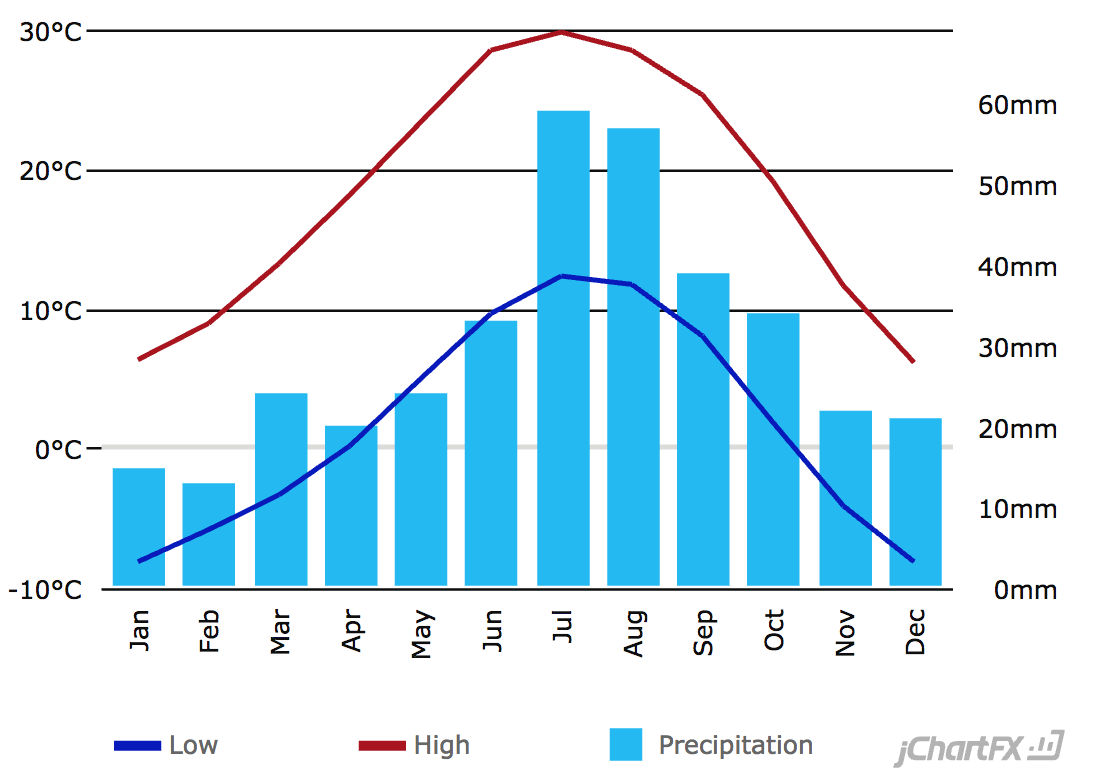
\includegraphics[width=12cm]{../figures/1_1_outside_source}
\end{figure}

We could tell that the min and max daily temperature agree with what we get from our data.

\begin{figure}[H]
\centering
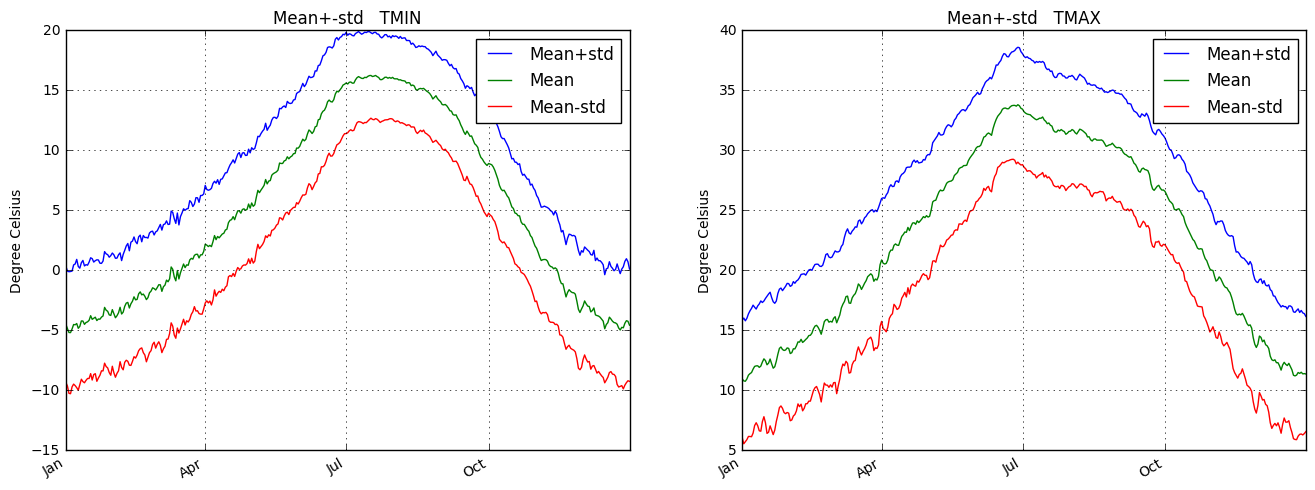
\includegraphics[width=15cm]{../figures/1_2_min_max_temperature}
\end{figure}

To compare the precipitation, we translate millimeter/day to millimeter/month. Although the precipitaion in some month like April and November has a little difference with the outside data, there is an agreement that the precipitation is distributed unevenly and seasonally, and most of the precipitation concentrate in the summer months.

\begin{figure}[H]
\centering
\begin{tabular}{cc}
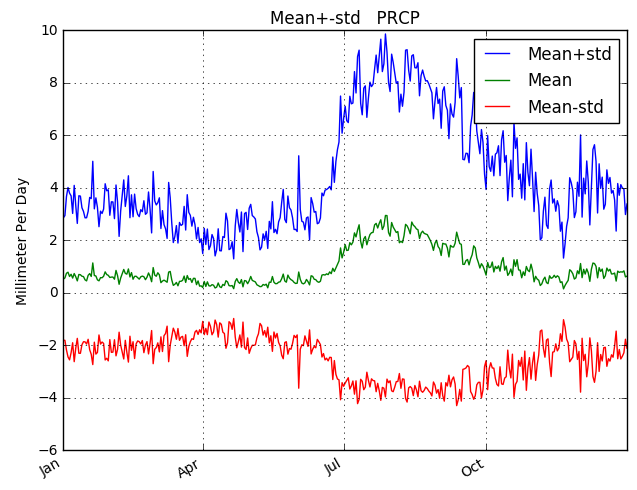
\includegraphics[width=7.5cm]{../figures/1_3_precipitation_daily} &
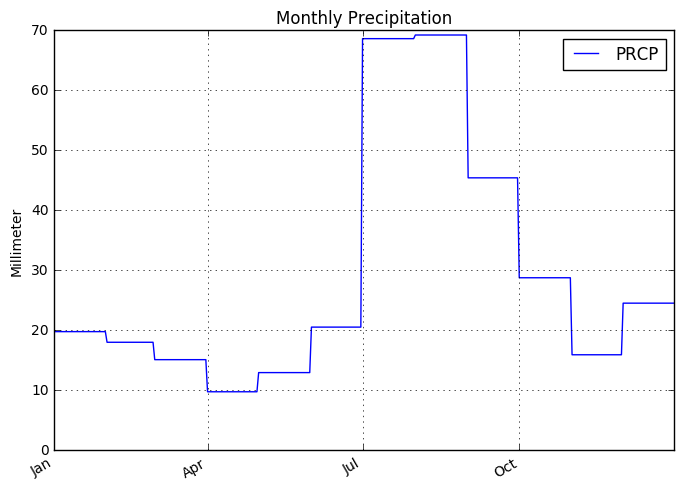
\includegraphics[width=7.5cm]{../figures/1_3_precipitation_monthly}
\end{tabular}
\end{figure}


\section*{PCA Analysis}
For each of the six meaurement, we compute the percentage of the variance explained as a function of the number of eigen-vectors used. \\

\subsection*{Percentage of Variance Explained}

We see that the top $6$ eigen-vectors explain $45\%$ of variance for TMIN, $59\%$ for TOBS and $50\%$ for TMAX.
We conclude that of the three, TOBS is best explained by the top 6 eigenvectors. This is especially true for the first eigen-vector which, by itself, explains $50\%$ of the variance. \\

\begin{figure}[H]
\centering
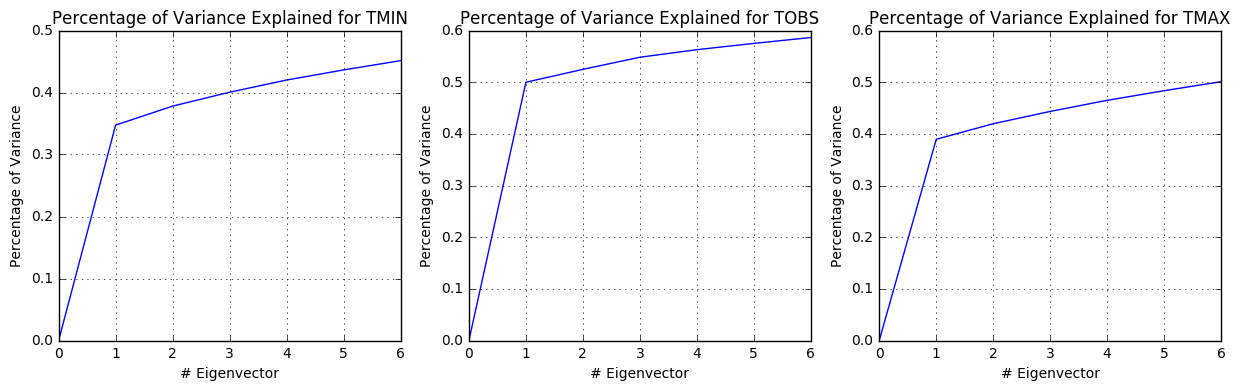
\includegraphics[width=15cm]{../figures/2_1_pca_temperature_explain}
\end{figure}

The top $6$ eigenvectors explain $9.5\%$ of the variance for PRCP and $16\%$ for SNOW. Both are low values. On the other hand the top 5 eigenvectors explain $76\%$ of the variance for SNWD. This means that these top $6$ eigenvectors capture most of the variation in the snow signals. It makes sense that SNWD would be less noisy than SNOW. That is because SNWD is a decaying integral of SNOW and, as such, varies less between days and between the same date on diffferent years. \\

\begin{figure}[H]
\centering
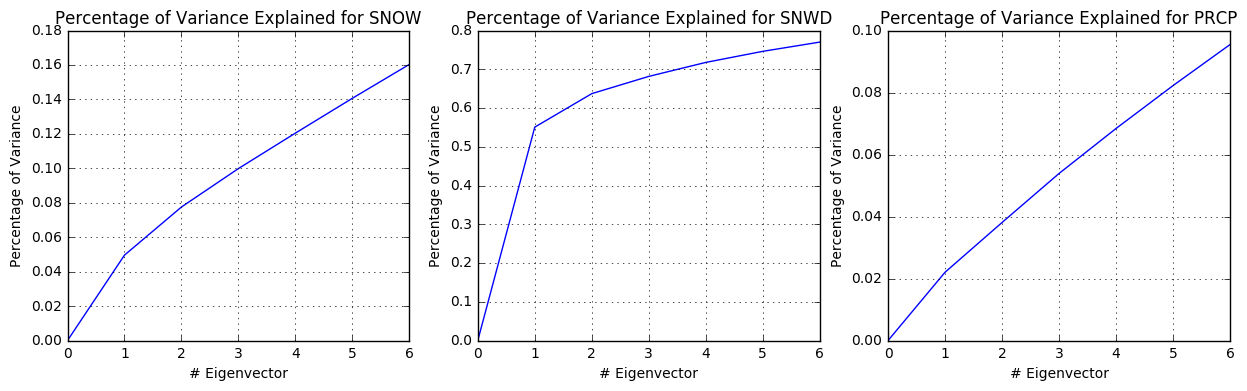
\includegraphics[width=15cm]{../figures/2_2_pca_snow_explain}
\end{figure}

Since SNWD can be well explained by the top eigenvectors, we will dig deeper into the PCA analysis for the snow depth SNWD.% and the observed temperature TOBS. 

\section*{Analysis of Snow Depth}
We analyze the eigen-decomposition for snow-depth using the first $5$eigen-vectors which explain $75\%$ of the variance. \\

First, we graph the mean and the top $5$ eigen-vectors.

\begin{figure}[H]
\centering
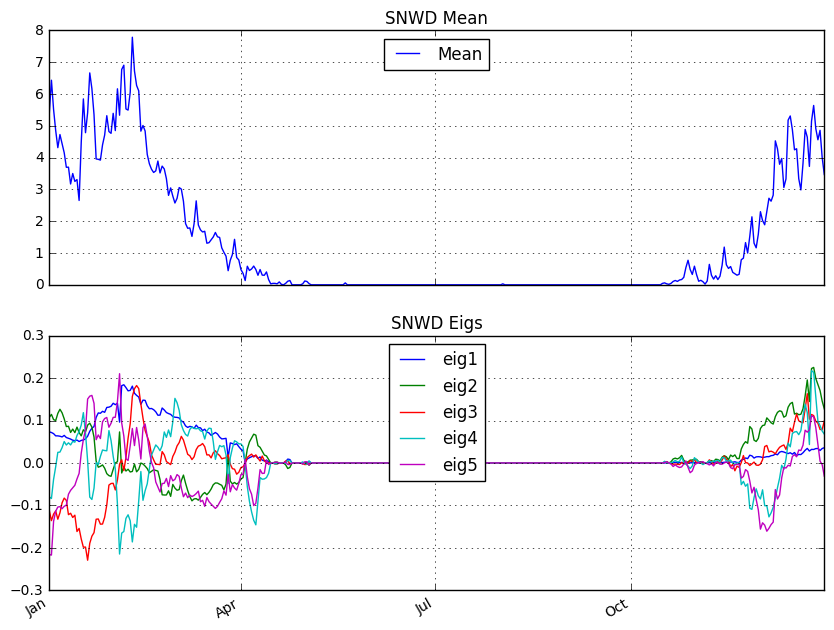
\includegraphics[width=15cm,height=8.17cm]{../figures/3_1_mean_eigen_vector}
\end{figure}

We observe that the snow season is from mid-november to the start of April, where the middle of February marks the peak of the snow-depth. Even in the snow season, it is a light snow instead of a heavy snow. \\

And then we interpret the eigen-functions. The first eigen-function (\textbf{eig1}) has a shape very similar to the mean function. The main difference is that the eigen-function is close to zero during october-december while the mean is not. The interpretation of this shape is that eig1 represents the overall amount of snow above/below the mean, but without changing the distribution over time.
\textbf{eig2},\textbf{eig3}, \textbf{eig4} and \textbf{eig5} are similar in the following way. They all oscilate between positive and negative values. In other words, they correspond to changing the distribution of the snow depth over the winter months, but they don't change the total (much). \\

They can be interpreted as follows:
\begin{itemize}
\item \textbf{eig2}: more snow in january and mid november-december; less snow in febuary-march.
\item \textbf{eig3}: less snow in january; more snow in febuary and december.
\item \textbf{eig4}: more snow in start january, mid febuary-march, and the end of december; less snow in start-mid febuary, start april and the end of november-start december.
\item \textbf{eig5}: more snow in mid january-mid febuary and the end of december; less snow in start january, mid febuary-start april, and mid november-start december.
\end{itemize}

\subsection*{Examples of reconstructions}
Here, we only use the first $3$ eigenvectors to reconstruct the original snow depth. Coeff are those coeffectives associate with these eigenvectors. 

\subsubsection*{Coeff1}

\begin{figure}[H]
\centering
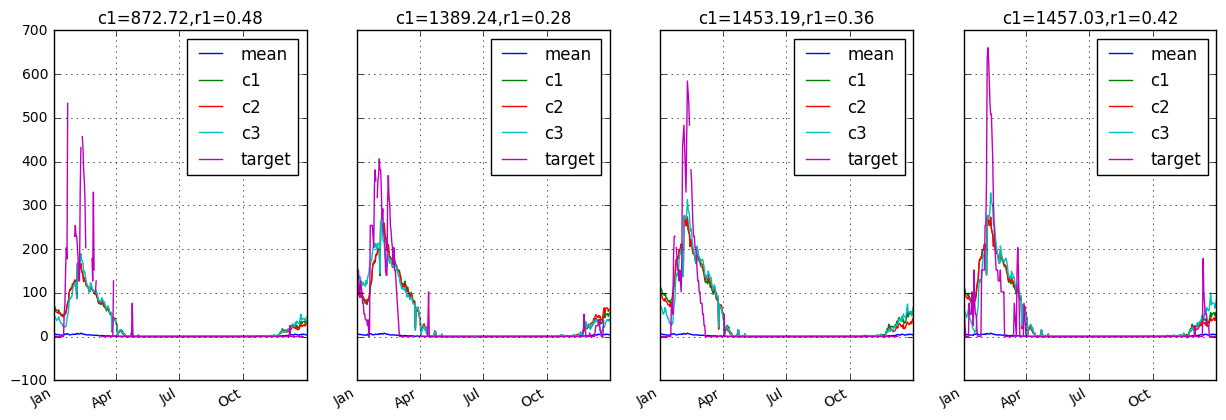
\includegraphics[width=15cm]{../figures/3_2_coeff1_smallest}
\caption{The smallest coeff1 for eig1}
\end{figure}

\begin{figure}[H]
\centering
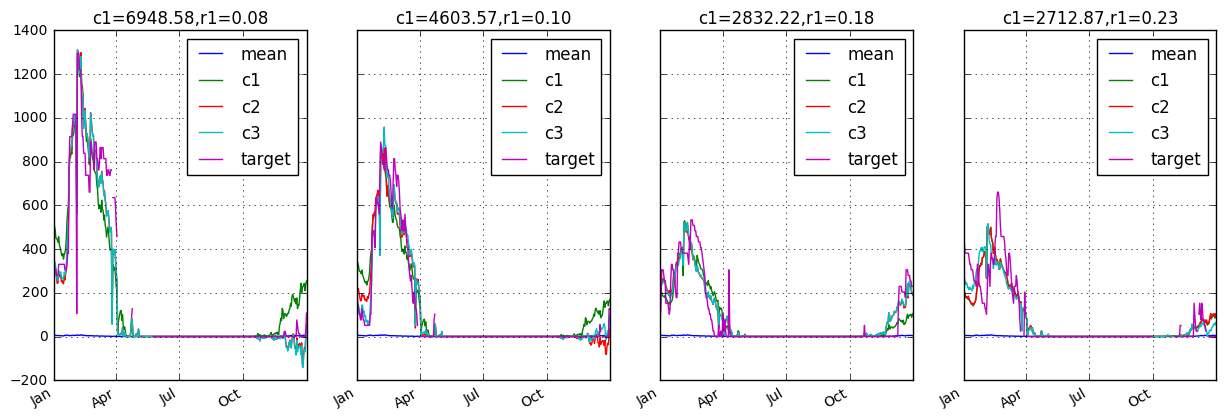
\includegraphics[width=15cm]{../figures/3_2_coeff1_largest}
\caption{The largest coeff1 for eig1}
\end{figure}

Large values of coeff1 correspond to a heavy snow in feb. Small values for coeff1 correspond to an light snow in feb. No negative values of coeff1 are founded when we restrict the residual1(using mean and eig1 only) to be smaller than $0.5$. The interpretation of no negative values is that the eig1 represents the overall amount of snow depth, and this shape will still remain with the changing stations and years.


\subsubsection*{Coeff2}

\begin{figure}[H]
\centering
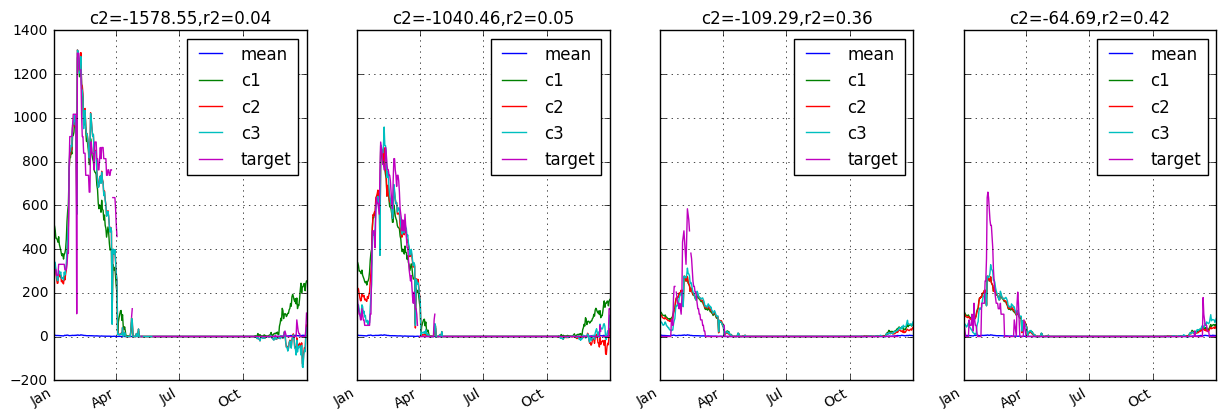
\includegraphics[width=15cm]{../figures/3_2_coeff2_smallest}
\caption{The smallest coeff2 for eig2}
\end{figure}

\begin{figure}[H]
\centering
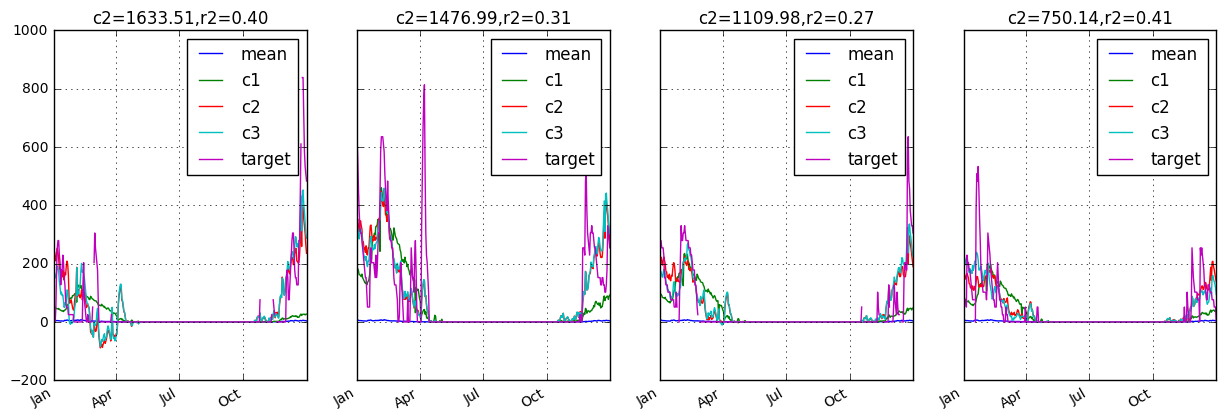
\includegraphics[width=15cm]{../figures/3_2_coeff2_largest}
\caption{The largest coeff2 for eig2}
\end{figure}

Large positive values of coeff2 correspond to an early snow season(Snow begins to fall on november-january). Small negative values for coeff2 correspond to a late snow season(Snow begins to fall on mid january-march).

\subsubsection*{Coeff3}

\begin{figure}[H]
\centering
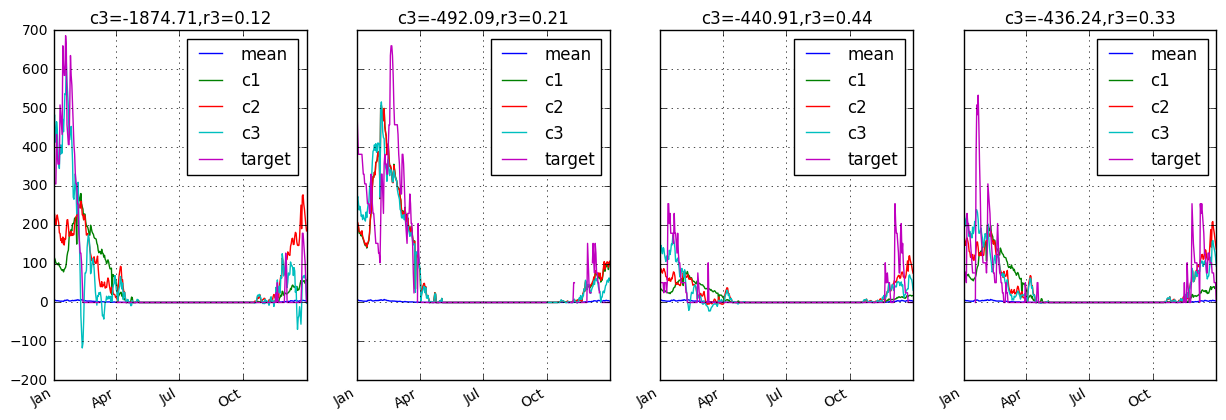
\includegraphics[width=15cm]{../figures/3_2_coeff3_smallest}
\caption{The smallest coeff3 for eig3}
\end{figure}

\begin{figure}[H]
\centering
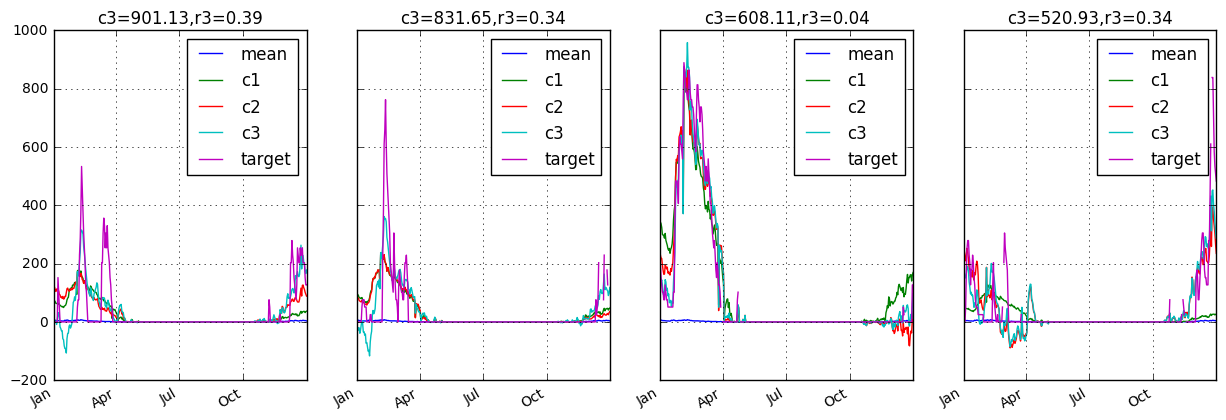
\includegraphics[width=15cm]{../figures/3_2_coeff3_largest}
\caption{The largest coeff3 for eig3}
\end{figure}

Large positive values of coeff3 correspond to a snow season with two spikes: one in the end of december, the other in the febuary. Negative values of coeff3 correspond to a season with a single peak at the start of Jan.


\subsection*{The variation in SNWD}
In the section above, we use the total amount of snow depth from different stations. We now estimate the relative importance of location-to-location variation relative to year-by-year variation. \\

These are measured using the fraction by which the variance is reduced when we subtract from each station/year entry the average-per-year or the average-per-station respectively. \\

The equation for the fraction is showed below:
\begin{equation*}
\textrm{fraction explained by station} = \frac{\textrm{total RMS - RMS removing mean-by-station}}{\textrm{total RMS}}
\end{equation*}
\begin{equation*}
\textrm{fraction explained by year} = \frac{\textrm{total RMS - RMS removing mean-by-year}}{\textrm{total RMS}}
\end{equation*}

Here are the results: \\

\textbf{coeff\_1} \\
total MS = $557.47$ \\
MS removing mean-by-station=$396.03$, fraction explained=$28.96\%$ \\
MS removing mean-by-year=$455.21$, fraction explained=$18.34\%$ \\

\textbf{coeff\_2} \\
total MS = $219.39$ \\
MS removing mean-by-station=$180.90$, fraction explained=$17.54\%$ \\
MS removing mean-by-year=$177.52$, fraction explained=$19.08\%$ \\

\textbf{coeff\_3} \\
total MS = $167.95$ \\
MS removing mean-by-station=$165.16$, fraction explained=$1.66\%$ \\
MS removing mean-by-year=$136.59$, fraction explained=$18.67\%$ \\

For the coeff\_1, it dues more to the location-to-location variation. Which the coeff\_2, and coeff\_3 due more to the year-by-year variation. However, both the location-to-location variation and the year-by-year variation are not the main source for the coeff RMS. We think the reason for this is the light snow in this region. The change in snow depth can be easily influenced by the random factors.



\section*{Analysis of TOBS}
Because TOBS is also a measurement that can be well reconstructed using the PCA method. We want to explore further about TOBS.\\

We then graph the mean and the top $5$ eigen-vectors.

\begin{figure}[H]
\centering
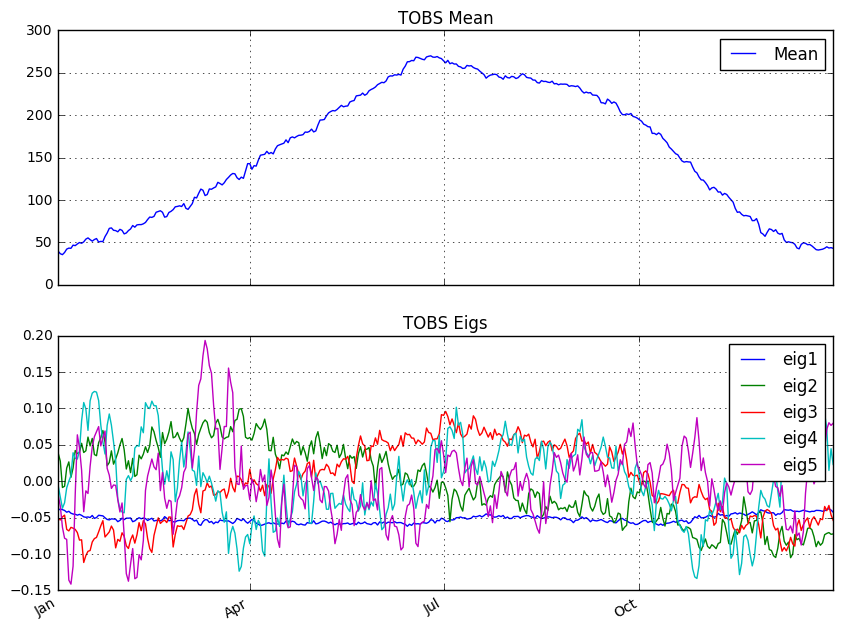
\includegraphics[width=15cm,height=8.17cm]{../figures/4_1_mean_eigen_vector}
\end{figure}

We observe that the temperature eigenvectors are changing dramatically through the years. We the revert to the analysis of PRCP. \\



\section*{Analysis of PRCP}

We then graph the mean and the top $5$ eigen-vectors.

\begin{figure}[H]
\centering
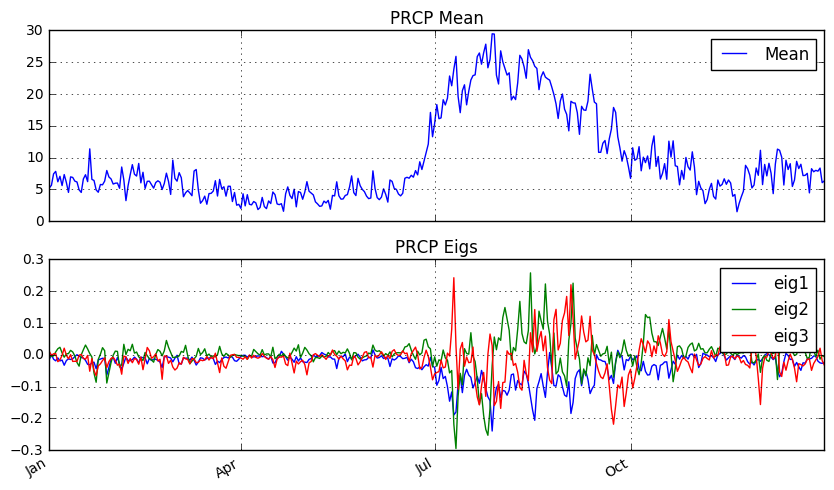
\includegraphics[width=15cm,height=8.17cm]{../figures/5_1_mean_eigen_vector}
\end{figure}

We observe that the precipitation mainly concentrate in the summer season. The eigenvectors then have a irregular oscillation in the summer season.\\



%http://www.matrix67.com/blog/archives/116
%\rule{\textwidth}{0.01in}
%%%%%%%%%%%%%%%%%%%%%%%%%%%%%%%%%%%%%%%%%%%%%%%%%%%%%%%%%%%%%%%%%%%%%%%%%%%%%%%%%%%%%%%%%%%
\end{document}

